\begin{figure}[h]
  \centering
  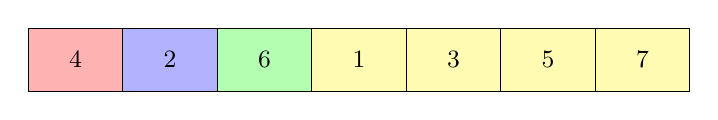
\begin{tikzpicture}
    \def\w{1.2} 
    \def\h{0.8}   

    \foreach \key/\col [count=\i from 0] in {4/red!30, 2/blue!30, 6/green!30,
                                             1/yellow!30, 3/yellow!30,
                                             5/yellow!30, 7/yellow!30}{
      \draw[fill=\col] (\i*\w,0) rectangle ++(\w,\h);
      \node at (\i*\w+0.5*\w,0.5*\h) {\small \key};
    }
  \end{tikzpicture}
  \caption[Plain BST Insertion Example]{Plain BST insertion (level-order) memory blocks.}
  \label{fig:plainmem}
\end{figure}
